\section{Code Transformation}\label{sec:trans}

\subsection{Formalization of the Transformation Rules}

% old
% In this section, we describe formalization of the transformation rule
% for distributed DL traininig with set of code examples and formal notions
% related to them.
% There are two main points in design of the formalization.
% First, we informally understand the code transformation rule as methods to
% \textit{select} the parts of codes to modify and \textit{construct} new code by 
% reusing parts of the selected code.
% To automate the transformation process, we need code transformation in a form 
% that is implements above selection and construction.
% Second, as mentioned earlier, to correctly transform tranining codes with different
% API patterns, we must apply different transformation rules.
% The formalization should also describe different transformation rules
% for different API patterns.
% 
% In this end, we define the formal transformation rule as a set of
% function that takes ASTs as input and returns ASTs as output.
% We call these functions as \textit{transform functions}.
% We define a set of transform functions for each training API pattern,
% defining total of four sets transform functions.
% For the selection and construction of code parts,
% we use \textit{pattern matching} as an argument of the transform function;
% given an AST as input, the transform function will first match the
% input against the argument pattern, then only proceed to apply itself
% when the pattern matching is successful.

% todo: graphical issue in this figure image
\begin{figure}[ht!]
    \centering
    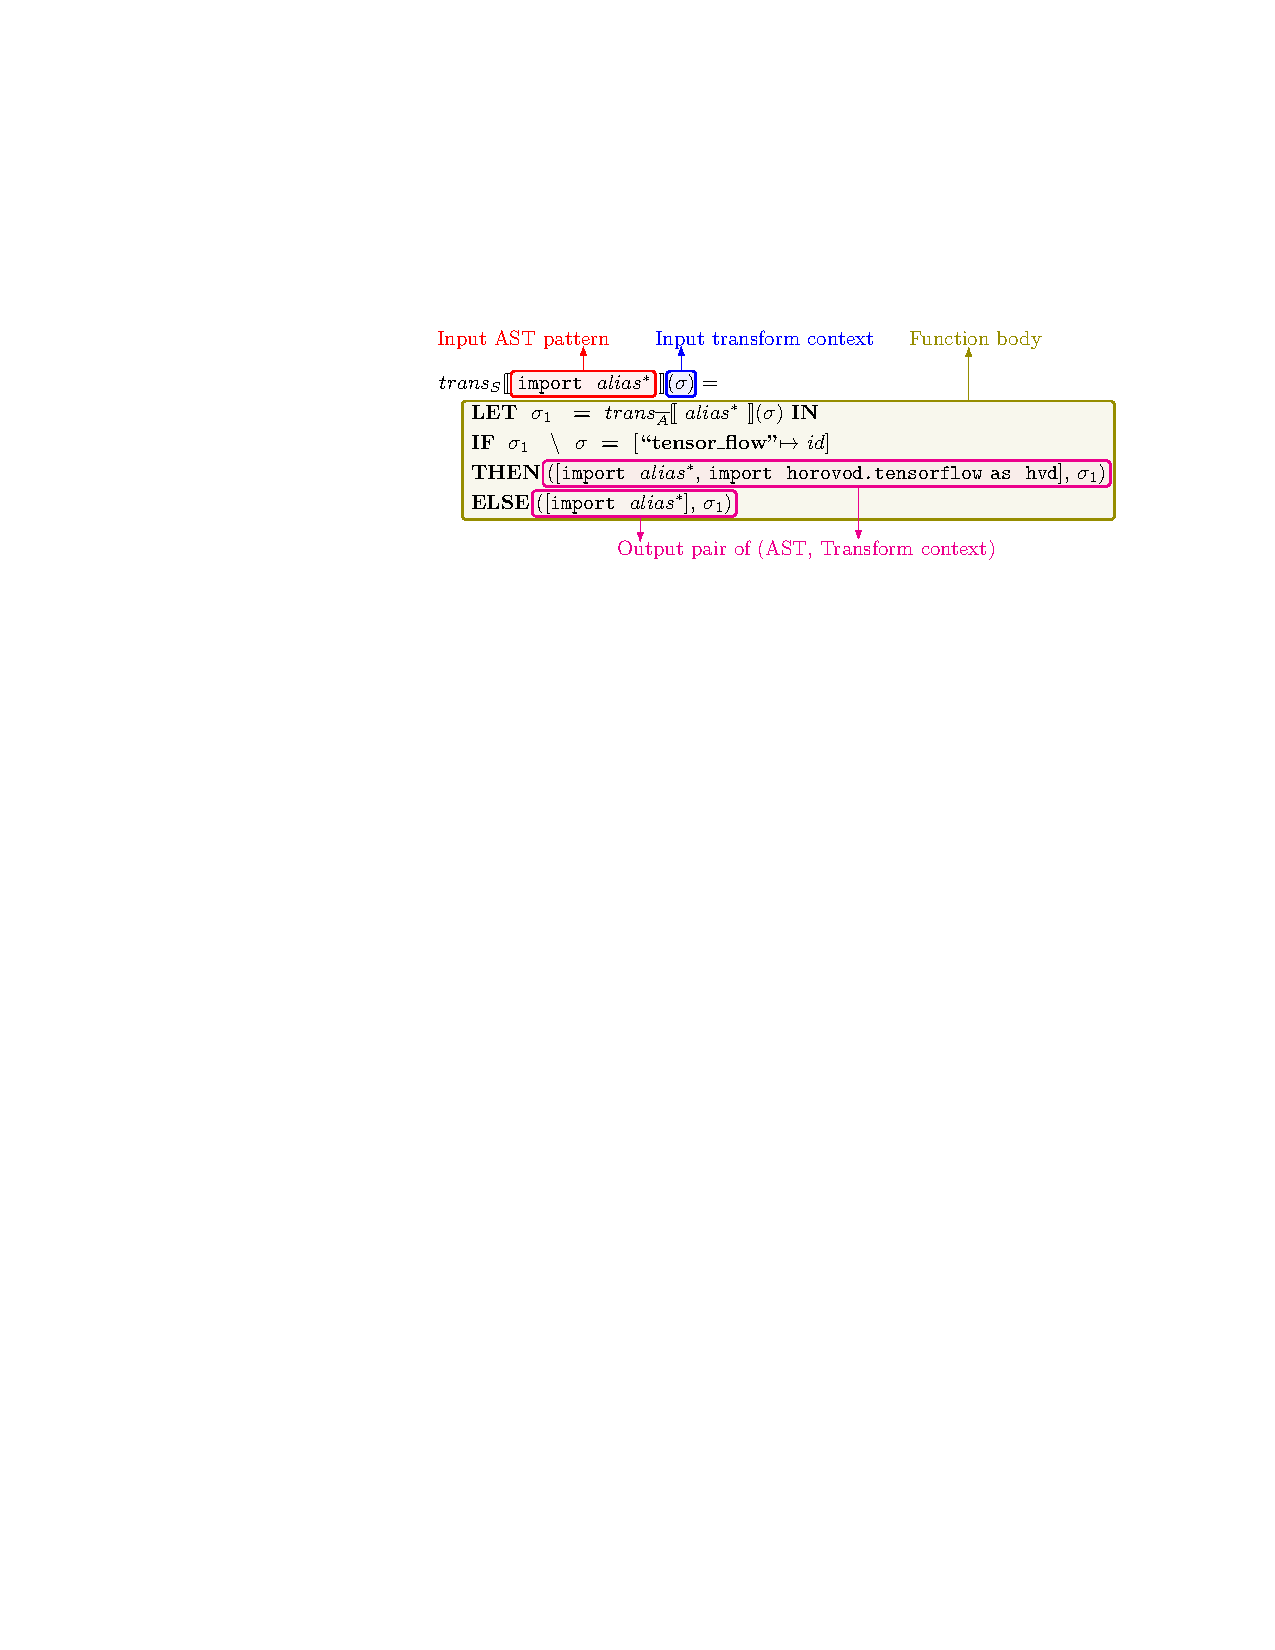
\includegraphics[width=0.7\textwidth]{transfn_expl.pdf}
    \caption{Explanation of Transform Function Description}
    \label{fig:trans:fnexpl}
\end{figure}

% new
We formalize the transformation rule as \textit{transform functions}.
% F : (AST, ctx) -> (AST, ctx)
Transform functions are the pure functions that takes an input AST and
returns the output ASTs.
% AST expl
The input AST corresponds to the input single-GPU model,
and the output AST corresponds to the transformed multi-GPU model.
% transform context expl
However, the transform functions cannot utilize the contextual information
by only getting ASTs as inputs.
For instance, the transform function inserts method call statements for
{\tt Optimizer} or {\tt GradientTape} instance.
Without knowing the instance name that appeared in previous function calls,
the transform function cannot add the correct code for the method call.
To solve this problem, the transform functions gets and returns
the \textit{transform context} objects as inputs and outputs.
The transform context is a finite mapping from strings to identifiers, which
context stores arbitrary identifiers from the code and propagate them to the 
next function calls.
When transform functions are sequentially applied to sequence of ASTs, 
the output transform context from the previous call is given as the input
to the next tranform function call.
By this method, the tranform functions can utilize contextual information
during transformation.

% transform function format expl
We describe the transform function in terms of the formal notation illustrated
in the figure~\ref{fig:trans:fnexpl}.
The figure~\ref{fig:trans:fnexpl} describes the part of transform function that
takes an {\tt import} statement AST as an input and returns the list of 
two {\tt import} statements as the output.
The function uses the AST pattern in the input parameter position.
The input AST pattern means that the function only applies the function body
to the ASTs that matches the pattern. 
The function also takes the transform context $\smodenv$ as an input.
Given the inputs, the function body specifies the output AST and the output
transform context.
We use complex expressions such as LET-IN or IF-THEN-ELSE to 
check and specify conditions to return different outputs.
In the figure~\ref{fig:trans:tnexpl}, for instance, 
the function body uses IF-THEN-ELSE expression to check if the {\tt import}
statement imports the {\tt tensorflow} module and return different
results according to the condition.

\begin{figure}[ht!]
  \centering
  \begin{subfigure}[t]{0.48\textwidth}
    \begin{lstlisting}[language=Python]
import tensorflow as tf

dataset = ...
model = ...
optim = tf.optimizers.Adam(0.001) 

for (x, y) in dataset.take(10000):
  with tf.GradientTape() as tape:
    pred = model(x)
    loss_value = loss(y, pred)\end{lstlisting} 
    \caption{Original DL training code}
  \end{subfigure}
  \hspace{5mm}
  \begin{subfigure}[t]{0.48\textwidth}
    \begin{lstlisting}[language=Python]
import tensorflow as tf
import horovod.tensorflow as hvd

dataset = ...
model = ...
optim = tf.optimizers.Adam(0.001 * hvd.size()) 

for (x, y) in dataset.take(10000):
  with tf.GradientTape() as tape:
    pred = model(x)
    loss_value = loss(y, pred) 
  tape = hvd.DistributedGradientTape(tape)\end{lstlisting}
    \caption{Distributed DL training code}
  \end{subfigure}
  \caption{Example of original DL model code transformed into the distributed model}
  \label{fig:trans:ex}
\end{figure}

We explain the details on the transform functions by code example in
the figure \ref{fig:trans:ex}. The figure is the pair of single-GPU model
and the corresponding multi-GPU model.
There are three modified parts of the code. 
First, an import statement for the Horovod module is added in the line 2. 
The statement is added right after the {\tt tensorflow} module import statement.
Second, in the line 6, the argument of the {\tt Optimizer} instance constructor
is modified. The new argument expression multiplies {\tt hvd.size()} 
onto the original argument expression.
Third, in the line 12, the statement that assigns the variable {\tt tape}
is added. The assignment wraps the original {\tt GradientTape} object with
the Horovod library function, {\tt hvd.DistributedGradientTape}.
Except the above mentioned parts, the original code is not modified.     

\begin{figure}[ht!]
  \centering
  \begin{subfigure}[t]{0.48\textwidth}
    \begin{lstlisting}[language=Python]
import tensorflow as tf\end{lstlisting}
    \caption{Original DL training code: only TensorFlow module is imported.}
  \end{subfigure}
  \hspace{5mm}
  \begin{subfigure}[t]{0.48\textwidth}
    \begin{lstlisting}[language=Python]
import tensorflow as tf
import horovod.tensorflow as hvd\end{lstlisting}
    \caption{Distributed DL training code: Horovod module import statement is added.}
  \end{subfigure}
  \caption{Code examples}
  \label{fig:trans:ex01}
\end{figure}

\begin{figure}[ht!]
  \centering
  \noindent
  \begin{tabular}{l}
   %\typdesc{\fkstmt& : & \dstmt ~ $\rightarrow$ ~ \dmodenv ~ $\rightarrow$ ~ (\dstmt ~ list ~ $\times$ ~ \dmodenv)}\\
   \tstmt{\kimport ~ \mul{\nalias}}{\smodenv} = \\
    \inden \ktlet ~ \smodenvsubs{1} ~ \kteq ~ \taalias{\mul{\nalias}}{\smodenv} \ktin \\
    \inden \ktif ~ \smodenvsubs{1} ~ \envsub ~ \smodenv ~ \kteq ~ [\tflow $\mapsto$ \nid]\\ 
    \inden\ktthen \\
    \inden\hspace{1em} ([\kimport ~ \mul{\nalias},
	  \kimport ~ {\tt horovod.tensorflow} \kas ~ {\tt hvd}], \smodenvsubs{1})\\
    \inden \ktelse~([\kimport ~ \mul{\nalias}], \smodenvsubs{1})
  \end{tabular}\\\vpar
  \caption{Transform function: adding Horovod module import statement}
  \label{fig:trans:fn01}
\end{figure}


Figure \ref{fig:trans:ex01} is the first transformed part of the code, and
the figure \ref{fig:trans:fn01} describe the transform function that
applies the transformation in the figure \ref{fig:trans:ex01}.
The input AST pattern matches the {\tt import} statements; 
The transform function should identify the input statement that imports 
the TensorFlow module, then outputs the list of two statements, 
which are the original input import statement and the new import statement 
for the Horovod module. 
The transform function should be able to recognize that the input import
statement actually imports the TensorFlow module.
To acheive this, the transform function utilzes the transform context.
The second and third lines of the figure~\ref{fig:trans:fn01}
compare $\smodenv$, the transform context
before the input statement, with $\smodenvsubs{1}$, the transform context
just after the input statement, to check if the input statement
imports the TensorFlow module.  
If the difference between $\smodenv$ and $\smodenvsubs{1}$ includes the
{\tt tensorflow} module identifier,
then the transform function adds the {\tt horovod.tensorflow} {\tt import} 
statement to the output AST.

\pagebreak
\begin{figure}[ht!]
  \centering
  \begin{subfigure}[t]{0.48\textwidth}
    \begin{lstlisting}[language=Python]
optim = tf.optimizers.Adam(0.001)\end{lstlisting}
    \caption{Original DL training code}
  \end{subfigure}
  \hspace{5mm}
  \begin{subfigure}[t]{0.48\textwidth}
    \begin{lstlisting}[language=Python]
optim = tf.optimizers.Adam(0.001 * hvd.size())\end{lstlisting}
    \caption{Distributed DL training code}
  \end{subfigure}
  \caption{Code examples}
  \label{fig:trans:ex02}
\end{figure}

\begin{figure}[ht!]
  \centering
  \begin{tabular}{l}

  \typdesc{\fkstmt& : & \dstmt ~ $\rightarrow$ ~ \dmodenv ~ $\rightarrow$ ~ (\dstmt ~ list ~ $\times$ ~ \dmodenv)}\\

  \tstmt{\nidsubs{r} \oassign \nexprsubs{1} \sparen{\nexprsubs{11} ... \nexprsubs{1n}} }{\smodenv} = \\

  \inden \ktif ~ \nexprsubs{1} \ktsubtysubs{\smodenv} ~ {\tt tensorflow.keras.optimizers.Optimizer}\\
  \inden \ktthen \\

  \inden\inden ([\nidsubs{r} \oassign \nexprsubs{1} \sparen{\nexprsubs{11}
  {\tt * hvd.size()} ... \nexprsubs{1n}}], \smodenv[\optmizer $\mapsto$ \nidsubs{r}])\\

  \end{tabular}
  \caption{Transform function: scaling the Optimizer instance argument}
  \label{fig:trans:fn02}
\end{figure}


The figure \ref{fig:trans:ex02} illustrates the second part of the transformed 
code, and the figure \ref{fig:trans:fn02} describes the transform function 
that applies the transformation in figure \ref{fig:trans:ex02}.
The learning rate argument for the {\tt Optimizer} class constructor is 
multiplied by the expression {\tt hvd.size()}. 
To apply the transformation, the transform function must first recognize a
assign statement that creates an {\tt Optimizer} instance.
One caveat here is that the {\tt Optimizer} instance can be 
created by not only TensorFlow library APIs, but also
user-defined class constructors. We utilize the class inheritance information to
recognize the constructors that creates any subclasses of the {\tt Optimizer}
class. 
After identifying the {\tt Optimizer} class assign statement, 
the transform function modifies the argument expression of the
constructor call.
The transform function would take the original argument expression,
then create a new expression that multiplies {\tt hvd.size()}
To modify the argument expression, the function body utilizes the AST pattern
variable $\nexprsubs{11}$ in the input AST pattern.
The pattern variable $\nexprsubs{11}$ will match {\tt 0.001} in the figure
\ref{fig:trans:ex02}(a).
In the output AST, the modified argument expression 
$\nexprsubs{11} {\tt * hvd.size()}$ will expand to {\tt 0.001 * hvd.size()}.

\begin{figure}[ht!]
  \centering
  \begin{subfigure}[t]{0.48\textwidth}
    \begin{lstlisting}[language=Python]
for (x, y) in dataset.take(10000):
  with tf.GradientTape() as tape:
    pred = model(x)
    loss_value = loss(y, pred)\end{lstlisting} 
    \caption{Original DL training code}
  \end{subfigure}
  \hspace{5mm}
  \begin{subfigure}[t]{0.48\textwidth}
    \begin{lstlisting}[language=Python]
for (x, y) in dataset.take(10000):
  with tf.GradientTape() as tape:
    pred = model(x)
    loss_value = loss(y, pred) 
  tape = hvd.DistributedGradientTape(tape)\end{lstlisting}
    \caption{Distributed DL training code}
  \end{subfigure}
  \caption{Example of original DL model code transformed into the distributed model}
  \label{fig:trans:ex03}
\end{figure}

\begin{figure}[ht!]
  \centering
  \begin{tabular}{l}
  \typdesc{\fkstmt& : & \dstmt ~ $\rightarrow$ ~ \dmodenv ~ $\rightarrow$ ~ (\dstmt ~ list ~ $\times$ ~ \dmodenv)}\\
  \tstmt{\kwith ~ \mul{\nwithitem} ~ \kcolon ~ \mul{\nstmt}}{\smodenv} = \\
  \inden \ktlet ~ \mul{\nwithitem}$'$, \smodenvsubs{1} \kteq ~ \twwithitem{\mul{\nwithitem}}{\smodenv} \ktin \\
  \inden \ktlet ~ \mul{\nstmt}$'$, \smodenvsubs{2} \kteq ~ \tsstmt{\mul{\nstmt}}{\smodenvsubs{1}} \ktin \\
  \inden \ktif ~ \smodenvsubs{1} \envsub ~ \smodenv ~ \kteq ~ [\gtape $\mapsto$ \nid] ~ \ktthen\\
  \inden\inden ([\kwith ~ \mul{\nwithitem}$'$ ~ \kcolon ~ \mul{\nstmt}$'$, \\
  \inden\inden \nid ~ \oassign {\tt hvd.DistributedGradientTape(\nid)}], \smodenvsubs{2})\\
  \inden \ktelse ~ ([\kwith ~ \mul{\nwithitem}$'$ ~ \kcolon ~ \mul{\nstmt}$'$], \smodenvsubs{2})
\end{tabular}\\\vpar
  \caption{Transform function: wrapping GraidentTape instance with Horovod API}
  \label{fig:trans:fn03}
\end{figure}

Figure \ref{fig:trans:ex03} is the third transformed part of the code, and
the figure \ref{fig:trans:fn03} describes the transform function responsible 
of the transformation of figure \ref{fig:trans:ex03}.
The new assign statement is added after the {\tt with} statement body end.
To apply this transformation, the transform function must first identify
a with statement that creates a new {\tt GradientTape} instance. 
The transform function utilizes the transform context to recognize a
with statement that creates a new {\tt GradientTape} instance. 
The transform function compares the input transform context with the 
transform context just after processing the with statement to check
whether the input with statement creates a {\tt GradientTape} instance.
Then, the transform function adds a new assign statement after the 
with statement, which wraps the variable with a
{\tt DistributedGradientTape} Horovod API.

% next subsection
\subsection{Transformation Rules for API Patterns}

%As mentioned earlier, different API patterns of the codes
%require different transformation rules to correctly transform them.
%To apply different transformation rules for different API pattern codes,
%we defined sets of transform functions each for trainng API patterns.
%This section explains the transform functions defined for each API patterns.

\subsubsection{Rules for the Session Pattern}

\begin{figure}[ht!]\centering
  \begin{subfigure}[t]{0.9\textwidth}
    \begin{lstlisting}[style=mpython]
optimizer = tf.train.MomentumOptimizer(learning_rate = 0.01)

with tf.Session() as sess:
    for step in range(num_epochs): 
        sess.run(optimizer, feed_dict)\end{lstlisting}
    \caption{Session pattern example}
    \label{fig:trans:sessiontrans:a}
  \end{subfigure}
  \hspace{5mm}
  \begin{subfigure}[t]{0.9\textwidth}
    \begin{lstlisting}[style=mpython]
optimizer = tf.train.MomentumOptimizer(learning_rate = 0.01 * hvd.size())
optimizer = hvd.DistributedOptimizer(optimizer)

with tf.Session() as sess:
    for step in range(num_epochs): 
        sess.run(optimizer, feed_dict)\end{lstlisting}
    \caption{Distributed Session pattern example}
    \label{fig:trans:sessiontrans:b}
  \end{subfigure}
  \caption{Example transformation of the Session pattern}
  \label{fig:trans:sessiontrans}
\end{figure}

\noindent
Figure \ref{fig:trans:sessiontrans} illustrates the required transformation of
the Session pattern using two code examples, \ref{fig:trans:sessiontrans:a} the
original training code and \ref{fig:trans:sessiontrans:b} its distributed
training version.
One of the primary transformations involves adjusting the learning rate
argument in the {\tt Optimizer} constructor call, which is achieved by
multiplying it by the number of GPUs.
The learning rate can be passed as the first positional argument in the
constructor call or as the keyword argument {\tt learning\_rate}.
The other transformation uses the Horovod-provided {\tt DistributedOptimizer}
instance instead of the original {\tt Optimizer} instance. 
To create the {\tt DisributedOptimizer} instance, the original {\tt Optimizer}
is passed as an argument to its constructor.

%To correctly transform Session pattern training codes into distributed 
%training codes, the {\tt Optimizer} instance must be modified.
%Figure \ref{fig:trans:sessiontrans} shows a pair of code examples
%illustrating the required transformation for Session pattern case.
%In line 1 of figure \ref{fig:trans:sessiontrans}(b),
%the learning rate argument is scaled by {\tt hvd.size()}.
%The learning rate can be specified by keyword argument {\tt learning\_rate}
%as the figure \ref{fig:trans:sessiontrans},
%or by the first positional argument.
%The transform function should be able to transform both of the cases.
%The transformation also adds a new statementd that wraps the 
%{\tt Optimizer} instance by {\tt DistributedOptimizer}.

\begin{figure}[ht!]\small
\noindent
  \begin{tabularx}{\textwidth}{X}
  \tstmt{\nidsubs{r} \oassign \nexprsubs{1} \sparen{\nexprsubs{11} ... \nexprsubs{1n} ~ \op{(\nidsubs{1} \oassign)} \nexprsubs{21} ... \op{(\nidsubs{k} \oassign)} \nexprsubs{2k}} }{\smodenv} = \\
  \inden \ktif ~ \nexprsubs{1} \ktsubtysubs{\smodenv} ~ {\tt tensorflow.keras.optimizers.Optimizer} ~ \ktthen\\
  \inden\inden \ktif ~ \nidsubs{i} ~ \kteq ~ {\tt learning\_rate} ~ \ktwhen ~ 1 $\leq$ i $\leq$ k ~ \ktthen\\
  \inden\inden\inden ([\nidsubs{r} \oassign \nexprsubs{1} \sparen{\nexprsubs{11} ... \nexprsubs{1n} ~ \op{(\nidsubs{1} \oassign)} \nexprsubs{21} ... \nidsubs{i} \oassign \nexprsubs{2i} {\tt * hvd.size()}\\
  \inden\inden\inden\inden ... \op{(\nidsubs{k} \oassign)} \nexprsubs{2k}}, \\
  \inden\inden\inden {\tt \nidsubs{r} = hvd.DistributedOptimizer(\nidsubs{r})}],\\
  \inden\inden\inden \smodenv[\optmizer $\mapsto$ \nidsubs{r}])\\

  \inden\inden \ktelse \\
  \inden\inden\inden ([\nidsubs{r} \oassign \nexprsubs{1} \sparen{\nexprsubs{11} {\tt * hvd.size()}... \nexprsubs{1n} ~ \op{(\nidsubs{1} \oassign)} \nexprsubs{21} ... \nidsubs{i} \oassign \nexprsubs{2i}\\
  \inden\inden\inden\inden ... \op{(\nidsubs{k} \oassign)} \nexprsubs{2k}}, \\
  \inden\inden\inden {\tt \nidsubs{r} = hvd.DistributedOptimizer(\nidsubs{r})}], \\
  \inden\inden\inden\smodenv[\optmizer $\mapsto$ \nidsubs{r}])\\

\end{tabularx}
  \caption{Session pattern transform function: Optimizer learning rate scaling and wrapping}
  \label{fig:trans:sessrule}
\end{figure}

Figure \ref{fig:trans:sessrule} shows the essential rule for the Session pattern,
which conducts the two transformations.
The transform rule matches an assignment statement that stores the result of a
function call expression into a variable.
Initially, the rule examines whether the callee function is the constructor of
either the {\tt Optimizer} class or any of its subclasses.
The predicate \ktsubtysubs{\smodenv} checks the subclass relation between two
classes using the class hierarchy analysis result.
Then, the rule adjusts the learning rate argument of the constructor call. 
Suppose the learning rate is passed as a keyword argument. 
In that case, the rule replaces the keyword argument value with the
multiplication of the original learning rate and the return value of {\tt
horovod.size()}.
Otherwise, the rule adjusts the first argument instead.
Following the adjustment of the learning rate, the rule adds a new statement:
$id_r\ =\ ${\tt hvd.DistributedOptimizer($id_r$)}. 
This statement replaces the original optimizer instance with a distributed
optimizer instance for any subsequent uses.

%Figure \ref{fig:trans:sessrule} formalizes the Sesison pattern transform 
%function. The transform function 
%matches assign statements that assign a result of function call expression.
%If an assign statement is matched, the pattern guard checks if the
%callee function is the {\tt Optimizer} instance constructor function.
%The pattern guard uses the subclass predicate \ktsubtysubs{\smodenv}
%to identify any expression that constructs the subclass of the TensorFlow
%{\tt Optimizer} class including user-defined classes.

%The third line of the transform function uses a branch to distinguish 
%whether the {\tt learning\_rate} argument is given as a keyword argument or not. 
%When the argument is given as a keyword argument,
%the transform function modifies the corresponding keyword argument expression
%as shown in the true branch in fourth line.
%When the argument is not given as a keyword argument,
%the transform function assumes that the first positional argument
%is the {\tt learning\_rate} argument and modifies it
%as shown in the eighth line.
%In either case, the transform function additionally returns a new
%assign statement that wraps the {\tt Optimizer} with
%{\tt hvd.DistributedOptimizer}.

\subsubsection{Rules for the MonitoredSession Pattern}
Figure~\ref{fig:trans:monsesstrans} describes an example transformation of the
MonitoredSession pattern code.
The {\tt MonitoredSession} constructor optionally requires a list of {\tt
SessionRunHook} objects as a keyword argument {\tt hooks}.
To ensure consistent global variable initialization of all processes in the
distributed training, the list needs to contain a {\tt
BroadcastGlobalVariableHook} object for the global variable broadcasting, as
shown in Figure~\ref{fig:trans:monsesstrans:b}.
The instance can be created by calling the constructor of the {\tt
BroadcastGlobalVariableHook} class with the ID of a source process.  
When starting the training, the hook broadcasts the initial global variable
parameters of the source to the other processes.\\

\begin{figure}
  \centering
  \begin{subfigure}[t]{0.8\textwidth}
    \begin{lstlisting}[style=mpython]
with tf.train.MonitoredTrainingSession(hooks=hooks) as mon_sess:
    while not mon_sess.should_stop():
        mon_sess.run()\end{lstlisting}
    \caption{MonitoredSession pattern example}
    \label{fig:trans:monsesstrans:a}
  \end{subfigure}
  \hspace{5mm}
  \begin{subfigure}[t]{0.8\textwidth}
    \begin{lstlisting}[style=mpython]
with tf.train.MonitoredTrainingSession(hooks=hooks.append(hvd.BroadcastGlobalVariablesHook(0)) as mon_sess:
    while not mon_sess.should_stop():
        mon_sess.run()\end{lstlisting}
    \caption{Distributed MonitoredSession pattern example}
    \label{fig:trans:monsesstrans:b}
  \end{subfigure}
  \caption{Example transformation of the MonitoredSession pattern}
  \label{fig:trans:monsesstrans}
\end{figure}


%\newpage
%To correctly transform the MonitoredSesion pattern code with the Horovod
%framework, 
%a hook for the variable broadcasting should be added to the
%{\tt MonitoredSession} object. 
%As in figure \ref{fig:trans:monsesstrans}, for example,
%the transformation appends {\tt BroadcastGlobalVariablesHook} to the
%{\tt hooks} arguments of the {\tt MonitoredSession} constructor call.
\vspace{-1em}

\begin{figure}[ht!]\small
 \noindent
  \begin{tabular}{l}
    %\typdesc{\fkstmt& : & \dstmt ~ $\rightarrow$ ~ \dmodenv ~ $\rightarrow$ ~ (\dstmt ~ list ~ $\times$ ~ \dmodenv)} \\
    \tstmt{\kwith ~ \mul{\nwithitem} ~ \kcolon ~ \mul{\nstmt}}{\smodenv} = \\
    \inden \ktlet ~ \mul{\nwithitem}$'$, \smodenvsubs{1} \kteq ~ \twwithitem{\mul{\nwithitem}}{\smodenv} \ktin \\
    \inden \ktlet ~ \mul{\nstmt}$'$, \smodenvsubs{2} \kteq ~ \tsstmt{\mul{\nstmt}}{\smodenvsubs{1}} \ktin \\

    \inden ([\kwith ~ \mul{\nwithitem}$'$ ~ \kcolon ~ \mul{\nstmt}$'$], \smodenvsubs{2})
  \end{tabular}\\[2ex]

  \begin{tabular}{l}
    %\typdesc{\fkwithitem & : & \dwithitem ~ $\rightarrow$ ~ \dmodenv ~ $\rightarrow$ ~ (\dwithitem ~ $\times$ \dmodenv)}  \\
    \twithitem{\nexprsubs{1} \sparen{\nexprsubs{11} ... \nexprsubs{1n} ~ 
                \op{(\nidsubs{1} \oassign)} \nexprsubs{21} ... 
                \op{(\nidsubs{k} \oassign)} \nexprsubs{2k}} {\tt as} \nidsubs{as} }{\smodenv} = \\

    \inden \ktif ~ \nexprsubs{1} \ktsubtysubs{\smodenv} {\tt tensorflow.train.MonitoredSession} ~ \ktthen \\
    \inden\inden \ktif ~ \nidsubs{i} ~ \kteq ~ {\tt hooks} ~ \ktwhen ~ 1 $\leq$ i $\leq$ k ~ \ktthen\\
    \inden\inden\inden(\nexprsubs{1} \sparen{\nexprsubs{11} ... 
              \nexprsubs{1n} ~ \op{(\nidsubs{1} \oassign)} \nexprsubs{21} \\
    \inden\inden\inden\inden ... \nidsubs{i} \oassign {\tt \nexprsubs{2i}.append(hvd.BroadcastGlobalVariablesHook(0))} \\
    \inden\inden\inden\inden ... \op{(\nidsubs{k} \oassign)} \nexprsubs{2k} }, \\
    \inden\inden\inden\inden \smodenv[ \msess $\mapsto$ \nidsubs{as}]) \\
  \end{tabular}\\\vpar
\caption{MonitoredSession pattern transform function: Modifying {\tt StopAtStepHook} instance}
  \label{fig:trans:monsessrule}
\end{figure}

%\vspace{-1em}

Figure \ref{fig:trans:monsessrule} formalizes the transform functions for the
MonitoredSession pattern.
The first transform function is responsible for matching {\tt with} statements
and transforming a list of the {\tt with\_item}, each of which represents a
variable and an assigned expression. 
The transform function denoted as \fkwwithitem~in line 2 applies the second
transform function \fkwithitem~to each {\tt with\_item}.
As a result, the first transform function returns a new {\tt with} statement
containing a list of the transformed {\tt with\_item}.
The second transform function transforms the {\tt with\_item}.
Among many forms of the {\tt with\_item}, the function matches those that
assign a function call result to a variable.
The second line checks whether the callee function of the {\tt with\_item} is a
constructor of the subclass of the {\tt MonitoredSession} class. 
If then, the transform function finds the keyword argument {\tt hooks} and
appends a {\tt BroadcastGlobalVariablesHook} object to the argument.\\

\subsubsection{Rules for the GradientTape pattern}\label{sec:grad}

\begin{figure}[ht!]
  \centering
  \begin{subfigure}[t]{0.8\textwidth}
    \begin{lstlisting}[style=mpython]
import tensorflow as tf

with tf.GradientTape() as tape:
    probs = model(images)
    loss_value = loss(labels, probs)

grads = tape.gradient(loss_value, model.trainable_variables)
opt.apply_gradients(zip(grads, model.trainable_variables))\end{lstlisting}
    \caption{GradientTape pattern example}
    \label{fig:trans:gtapetrans:a}
  \end{subfigure}
  \hspace{5mm}
  \begin{subfigure}[t]{0.8\textwidth}
    \begin{lstlisting}[style=mpython]
import tensorflow as tf
import horovod.tensorflow as hvd
hvd_broadcast_done = False

with tf.GradientTape() as tape:
    probs = model(images)
    loss_value = loss(labels, probs)
tape = hvd.DistributedGradientTape(tape)
grads = tape.gradient(loss_value, model.trainable_variables)
id_new = zip(grads, model.trainable_variables)
opt.apply_gradients(id_new)

global hvd_broadcast_done
if not hvd_broadcast_done:
    hvd.broadcast_variables([x[1] for x in id_new], root_rank=0,)
    hvd.broadcast_variables(opt.variables(), root_rank=0,)
    hvd_broadcast_done = True\end{lstlisting}
    \caption{Distributed GradientTape pattern example}
    \label{fig:trans:gtapetrans:b}
  \end{subfigure}
  \caption{Example transformation of the GradientTape pattern}
  \label{fig:trans:gtapetrans}
\end{figure}

\noindent
Figure \ref{fig:trans:gtapetrans} illustrates an example GradientTape pattern
code and its distributed version.  
For the distributed training, the model needs to utilize a {\tt
DistributedGradientTape} instance in training instead of the {\tt
GradientTape} instance, as shown in lines 8 and 9 in
Figure~\ref{fig:trans:gtapetrans:b}.
In addition, the model also needs to broadcast trainable global variables from
the root process to the others once after applying the gradients.
Lines 13 to 17 in Figure~\ref{fig:trans:gtapetrans:b} represent the code that
broadcasts the variables depending on the value of {\tt hvd\_broadcast\_done}.
Once finishing the broadcasting, the {\tt hvd\_broadcast\_done} is set to {\tt
False} to prevent further broadcasting.

%To correctly transform GradientTape pattern training codes,
%the {\tt GradientTape} instance should be modified for distributed training.
%As shown in line 8, figure \ref{fig:trans:gtapetrans}(b),
%the {\tt GradientTape} instance {\tt tape}
%is wrapped by a Horovod library API {\tt DistributedGradientTape}.
%In addition to modifying the {\tt GradientTape} instance,
%lines 13 to 17 add the variable broadcasting code after the
%{\tt apply\_gradients} method call.
%Note that the variable {\tt hvd\_broadcast\_done} is initialized as 
%{\tt False} at line 3. 
%Then line 17 sets the variable to {\tt True}, after the variable broadcasting
%is done.
%We use the boolean variable {\tt hvd\_broadcast\_done} in GrdientTape pattern
%model to ensure that variable broadcasting occurs exactly once.


\begin{figure}[ht!]\small
%\noindent
\begin{tabular}{l}
  \tstmt{\kwith ~ \mul{\nwithitem} ~ \kcolon ~ \mul{\nstmt}}{\smodenv} = \\
  \inden \ktlet ~ \mul{\nwithitem}$'$, \smodenvsubs{1} \kteq ~ \twwithitem{\mul{\nwithitem}}{\smodenv} \ktin \\
  \inden \ktlet ~ \nstmt$'$, \smodenvsubs{2} \kteq ~ \tsstmt{\mul{\nstmt}}{\smodenvsubs{1}} \ktin \\
  \inden \ktif ~ \smodenvsubs{1} \envsub ~ \smodenv ~ \kteq ~ [\gtape $\mapsto$ \nid] ~ \ktthen\\
  \inden\inden ([\kwith ~ \mul{\nwithitem}$'$ ~ \kcolon ~ \mul{\nstmt}$'$, \nid ~ \oassign {\tt hvd.DistributedGradientTape(\nid)}], \smodenvsubs{2})\\
  \inden \ktelse ~ ([\kwith ~ \mul{\nwithitem}$'$ ~ \kcolon ~ \mul{\nstmt}$'$], \smodenvsubs{2})
\end{tabular}
  \caption{GradientTape pattern transform function: utilizing the {\tt DistributedGradientTape} instance}
  \label{fig:trans:gtaperule}
\end{figure}

Figure \ref{fig:trans:gtaperule} formalizes the partial transform function for
utilizing the {\tt DistributedGradientTape} instance.
The transform function matches {\tt with} statements and updates the transform
context by transforming the list of {\tt with\_item}.
The updated transform context contains a mapping from the string {\tt
graident\_tape} to a variable \nid~if the {\tt with\_item} creates a {\tt
GradientTape} instance and assigns it to the variable.
Then, the function injects a new assignment statement, $\nid ~ \oassign~{\tt
hvd.DistributedGradientTape(\nid)}$, right after the {\tt with} statement,
which replaces the instance of the variable with a newly created {\tt
DistributedGradientTape} instance for further uses in subsequent statements.


\begin{figure}[ht!]\small
\noindent
\begin{tabular}{l}
  \tstmt{\nidsubs{r} \oassign \nexprsubs{1} \sparen{\nexprsubs{11} ... \nexprsubs{1n} ~ \op{(\nidsubs{1} \oassign)} \nexprsubs{21} ... \op{(\nidsubs{k} \oassign)} \nexprsubs{2k}} }{\smodenv} = \\
  \inden \ktif  ~ \smodenv(\optmizer) ~ \kteq ~ \nidsubs{t} ~ \ktand ~ \nexprsubs{1} ~ \kteq ~ {\tt \nidsubs{t}.apply\_gradients} ~ \ktthen\\
  \inden\inden \ktlet ~ \nidsubs{z} ~ \kteq ~ \newid ~ \ktin \\
  \inden\inden ([\nidsubs{z} ~ \oassign ~ \nexprsubs{11},\\
  \inden\inden \nidsubs{r} \oassign \nexprsubs{1} \sparen{\nidsubs{z} \nexprsubs{12} ... \nexprsubs{1n} ~ \op{(\nidsubs{1} \oassign)} \nexprsubs{21} ... \op{(\nidsubs{k} \oassign)} \nexprsubs{2k}} ,\\
  \inden\inden {\tt global hvd\_braodcast\_done},\\
  \inden\inden {\tt if not hvd\_broadcast\_done:} \\ 
  \inden\inden\inden [ {\tt hvd.broadcast\_variables([x[1] for x in \nidsubs{z}], root\_rank=0)}, \\
  \inden\inden\inden {\tt hvd.broadcast\_variables(\nidsubs{t}.variables(), root\_rank=0)}, \\
  \inden\inden\inden {\tt hvd\_broadcast\_done = True} ]\\
  \inden\inden ], \smodenv) \\
\end{tabular}
  \caption{GradientTape pattern transform function: broadcasting trainable global variables}
  \label{fig:trans:gtaperule2}
\end{figure}

Figure \ref{fig:trans:gtaperule2} formalizes the partial transform function
that appends the variable broadcasting code after the 
{\tt apply\_gradients} method call.
The function matches assignment statements that assign a function call result. 
When a variable $id_t$ stores the {\tt Optimizer} instance and the callee
function is {\tt $id_t$.apply\_gradients}, the transform function changes the
assignment statement and adds the variable broadcasting code.
The function injects a new assignment statement that stores the first argument
of the function call into a new variable $id_z$.
The first argument of the {\tt apply\_gradients} is an iterator of tuples that
contain pairs of gradients and trainable variables.
After the function call statement, the transform function injects a {\tt
global} statement to refer to the global broadcast flag variable {\tt
hvd\_broadcast\_done} and call statements guarded by the flag to broadcast
trainable variables stored in the tuples and {\tt opt.variables()}. 
The function also injects an assignment statement that sets the
global broadcast flag to {\tt True}.

%\pagebreak

   


\subsubsection{Rules for the Keras pattern}

\begin{figure}[ht!]\centering
  \begin{subfigure}[t]{0.8\textwidth}
  \begin{lstlisting}[style=mpython]
class ResNet(keras.Model):
    def __init__(self, block_list):
        ...

model = ResNet([2, 2, 2])

model.fit(x_train, y_train)\end{lstlisting}
  \caption{Keras pattern example}
    \label{fig:trans:keras:a}
  \end{subfigure}
  \hspace{3mm}
  \begin{subfigure}[t]{0.8\textwidth}
  \begin{lstlisting}[style=mpython]
class ResNet(keras.Model):
    def __init__(self, block_list):
        ...

model = ResNet([2, 2, 2])

callbacks=[hvd.callbacks.BroadcastGlobalVariablesCallback(0)]
model.fit(x_train, y_train,
          callbacks=callbacks)\end{lstlisting}
    \caption{Distributed Keras pattern example}
    \label{fig:trans:keras:b}
  \end{subfigure}
  \caption{Example transformation of the Keras Pattern}
  \label{fig:trans:keras}
\end{figure}

\noindent
Figure \ref{fig:trans:keras} illustrates an example transformation of the Keras
pattern.
The Keras pattern code usually defines a subclass of {\tt keras.Model}, such
as {\tt ResNet}, constructs a model as an instance of the class, and trains the
model by calling its {\tt fit} method inherited from {\tt keras.Model}.
To distribute the model's training with Horovod, the {\tt fit} method needs to
take a callback {\tt BroadcastGlobalVariablesCallback} as the keyword argument
{\tt callbacks}, shown in Figure~\ref{fig:trans:keras:b}.
When training starts, the callback ensures consistent initialization of all
processes by broadcasting initial global variable states from a source to the
other processes.

\begin{figure}[ht!]\small
\centering
\begin{tabular}{l}
  \tstmt{\nexprsubs{1} \sparen{\nexprsubs{11} ... \nexprsubs{1n} ~ \op{(\nidsubs{1} \oassign)} \nexprsubs{21} ... \op{(\nidsubs{k} \oassign)} \nexprsubs{2k}}}{\smodenv} = \\
  \inden \ktif ~ \nidsubs{m} ~ \kteq ~ \smodenv({\tmodel}) ~ \ktand ~ 
          \nexprsubs{1} ~ \kteq ~ {\tt \nidsubs{m}.fit} ~ \ktthen \\
  \inden\inden \ktif ~ \nidsubs{i} ~ \kteq ~ {\tt callbacks} ~ \ktwhen ~ 2 $\leq$ i $\leq$ k ~ \ktthen \\
  \inden\inden\inden ([{\tt cb = [hvd.callbacks.BroadcastGlobalVariablesCallback(root\_rank=0)},\\
  \inden\inden\inden ~ {\tt if hvd.rank() == 0: cb.append(\nexprsubs{2i})}, \\
  \inden\inden\inden ~ {\tt \nexprsubs{1} (\nexprsubs{11} ... \nexprsubs{1n}}
                              \op{(\nidsubs{1} \oassign)} \nexprsubs{21} ... 
                              \nidsubs{i} \oassign {\tt cb} ... 
                              \op{(\nidsubs{k} \oassign)} \nexprsubs{2k}{\tt )}], \smodenv) \\
  \inden\inden \ktelse \\
  \inden\inden\inden ([{\tt cb = [hvd.callbacks.BroadcastGlobalVariablesCallback(root\_rank=0)},\\
  \inden\inden\inden ~ {\tt \nexprsubs{1} (\nexprsubs{11}... \nexprsubs{1n}}
                              \op{(\nidsubs{1} \oassign)} \nexprsubs{21} ... 
                              \op{(\nidsubs{k} \oassign)} \nexprsubs{2k}
                              {\tt callbacks \oassign cb} {\tt )}],\\
                              \inden\inden\inden\inden\smodenv) \\
\end{tabular}
  \caption{Keras pattern transform function}
  \label{fig:trans:kerasrule}
\end{figure}

Figure \ref{fig:trans:kerasrule} formalizes the transform function for the
Keras pattern code.
The transform function matches function call statements for the {\tt fit}
method of model objects by checking whether the receiver object of the {\tt
fit} method call is an instance of a subclass of {\tt keras.Model}.
Then, if the function call already takes the {\tt callbacks} keyword argument,
the transform function changes the function call to three statements. 
The first and second statements create a temporary variable {\tt cb} for the
later use of the function call in the third statement.
Note that the second statement appends the original callbacks to the {\tt cb}
variable only when the {\tt hvd.rank()} is zero, which enables the original
callbacks to be called only on the one process.
If the keyword argument does not exist in the function call, the transform
function propagates the callback as the {\tt callbacks} keyword argument, shown
in Figure~ \ref{fig:trans:keras:b}.


